

% \subsection{Evaluation Setups}

\subsection{Experiment Setups}

\model{} is generally applicable to a wide spectrum tasks. As an early exploration, in this paper, we conduct experiments on mathematical reasoning problems where the learning signals are clear to define \ie, final answer is correct or wrong. We choose to evaluate on two widely used datasets GSM8K~\citep{gsm8k} and MATH~\citep{math}. For GSM8K, we utilize the whole test set while for MATH, due to computation constraints, we utilize a subset following the same procedure of~\cite{lightman2023let}. We evaluate the performance of predicting answers correctly for policy models. In addition, we calculate the average rollouts, represented by the number of nodes in the tree, as a measure of computational efficiency. We compare the performance of \model{} with a suite of proprietary model, including OpenAI's GPT-4 and GPT-3.5, Anthropic's Claude-2, as well as Google's PaLM-2 and the gemini model family. To ensure a fair and consistent evaluation, we employ CoT as our primary prompting method. Additionally, we conduct comparisons with strong open-source models, including Llama-2-70b~\citep{llama2} and WizardMath-70B-V1.0~\citep{wizardmath}. % For LLaMA-2 70B, we present results from few-shot prompting as well as zero-shot prompting for its SFT version, which was trained using CoT rationales and final answers. Wizardmath 70B has been trained on a diverse set of mathematical data generated by ChatGPT, employing both SFT and RLHF. We provide zero-shot prompting results.

%Means square errors and next token prediction accuracy are reported for evaluating value functions and \prm{}/\orm{}, respectively.
% \paragraph{Baseline Systems} We evaluate the performance of \model{} against a suite of proprietary model, including OpenAI's GPT-4 and GPT-3.5, Anthropic's Claude-2, as well as Google's PaLM-2 and the gemini model family. To ensure a fair and consistent evaluation, we employ CoT as our primary prompting method. We additionally report PAL~\citep{gao2023pal} prompting performance with GPT-4 as it demonstrates enhanced performance. Additionally, we conduct comparisons with strong open-source models, including LLaMA-2 70B~\citep{llama2} and Wizardmath 70B~\citep{wizardmath}. For LLaMA-2 70B, we present results from few-shot prompting as well as zero-shot prompting for its SFT version, which was trained using CoT rationales and final answers. Wizardmath 70B has been trained on a diverse set of mathematical data generated by ChatGPT, employing both SFT and RLHF. We provide zero-shot prompting results.

% The implementation details can be found in Appendix \ref{app:implementation}.


% \paragraph{Datasets} \model{} is generally applicable to a wide spectrum tasks. As an early exploration, in this paper, we conduct experiments on mathematical reasoning problems where the learning signals are clear to define \ie, final answer is correct or wrong. We choose to evaluate on two widely used datasets GSM8K~\citep{gsm8k} and MATH~\citep{math}. For GSM8K, we utilize the whole test set while for MATH, due to computation constraints, we utilize a subset following the same procedure of~\cite{lightman2023let}.
% \paragraph{Metrics} We evaluate the performance of predicting answers correctly for policy models. In the same time, we calculate the average rollouts, represented by the number of nodes in the tree, as a measure of computational efficiency. %Means square errors and next token prediction accuracy are reported for evaluating value functions and \prm{}/\orm{}, respectively.
% \paragraph{Baseline Systems} We evaluate the performance of \model{} against a suite of proprietary model, including OpenAI's GPT-4 and GPT-3.5, Anthropic's Claude-2, as well as Google's PaLM-2 and the gemini model family. To ensure a fair and consistent evaluation, we employ CoT as our primary prompting method. We additionally report PAL~\citep{gao2023pal} prompting performance with GPT-4 as it demonstrates enhanced performance. Additionally, we conduct comparisons with strong open-source models, including LLaMA-2 70B~\citep{llama2} and Wizardmath 70B~\citep{wizardmath}. For LLaMA-2 70B, we present results from few-shot prompting as well as zero-shot prompting for its SFT version, which was trained using CoT rationales and final answers. Wizardmath 70B has been trained on a diverse set of mathematical data generated by ChatGPT, employing both SFT and RLHF. We provide zero-shot prompting results.

% The implementation details can be found in Appendix \ref{app:implementation}.
% \subsection{Baseline Systems}
% We evaluate the performance of \model{} against a suite of proprietary model, including OpenAI's GPT-4 and GPT-3.5, Anthropic's Claude-2, as well as Google's PaLM-2 and the gemini model family. To ensure a fair and consistent evaluation, we employ CoT as our primary prompting method. We additionally report PAL~\citep{gao2023pal} prompting performance with GPT-4 as it demonstrates enhanced performance.

% Additionally, we conduct comparisons with strong open-source models, including LLaMA-2 70B~\citep{llama2} and Wizardmath 70B~\citep{wizardmath}. For LLaMA-2 70B, we present results from few-shot prompting as well as zero-shot prompting for its SFT version, which was trained using CoT rationales and final answers. Wizardmath 70B has been trained on a diverse set of mathematical data generated by ChatGPT, employing both SFT and RLHF. We provide zero-shot prompting results.

% We conduct our experiments on two math datasets, GSM8K~\citep{gsm8k} and MATH~\citep{math}.
% Our use LLaMa 2 70B~\citep{llama2} and WizardMath 70B V1.0~\citep{wizardmath} as our base models for GSM8K and MATH respectively.

% \subsection{Implementation Details}

We select Llama-2-70b as the policy model for the GSM8K dataset and WizardMath-70B-V1.0 for the MATH dataset. To construct the training dataset for the value function, \prm{} and \orm{}, we generate 50 trajectories for each prompt and construct the training target following Section~\ref{sec:critic}. Both \prm{} and \orm{} are initialized using the weights from the policy model, while the value function uses a smaller Llama-2-13b model, as we observed no performance gains from increasing the value function model size. In the design of \orm{}, tool usage is not incorporated for GSM8K. However, for MATH, we enhance \orm{} by incorporating tools like python sympy to assess the quality of a trajectory, in a manner similar to that described by \citet{gou2023tora}. The training employ a learning rate of 1e-6 and are trained for one epoch. For the fast rollout policy model, we opt for the Abel-002-7B model~\citep{abel} for both the GSM8K and MATH tasks for its high efficiency and superior performance. For the MCTS parameters, they are configured at different scales, as shown in Appendix \ref{app:implementation}. We set $\beta_{\text{value}}$, $\beta_{\text{PRM}}$, and $\beta_{\text{ORM}}$ all to 1.0.

% We set the MCTS parameters as follows: in GSM8K, $c=1$ for the small scale (\texttt{\#rollout}) and $1.5$ for the large scale, with $\alpha=1$. For $t=0$, $c_\text{min}(0)=10$ for the small scale and $40$ for the large scale, while for the rest of $t$, $c_\text{min}(t)=2$. We also set $c_\text{max}(0) = 10$ for the small scale and $40$ for the large scale, and for the remaining $t$, $c_\text{max}(t)=10$. The termination condition is based on sentence termination. In MATH, the parameters are $c=1$, $\alpha=1$, and for $t=0$, $c_\text{min}(0)=10$ for the small scale and $20$ for the large scale, while for the rest of $t$, $c_\text{min}(t)=3$. We set $c_\text{max}(0) = 10$ for the small scale and $20$ for the large scale, and for the remaining $t$, $c_\text{max}(t)=10$. The termination function is rule-based, checking if there are any formulations or calculations in the sentence. If there are, the option is terminated; otherwise, the option continues to extend.

For policy self-improving (\S \ref{sec:self_improve}), we train the policy model up to 3 epochs, setting batch size to 128, learning rate to $5\times 10^{-6}$ and minimal learning rate to $1\times 10^{-6}$.
Linear warm-up and decay is used with warm-up percent to be 10\%.
We perform early stopping based on a devset held out from the training instances.
For GSM8K experiments, we perform two rounds of self-improving, synthesizing 6.4k and 7.9k prompts\citep{yu2023metamath} respectively to obtain the corresponding MCTS outputs for training.
For MATH experiments, we only perform one round of self-improving due to limited computation resources, and 5.9k prompts are synthesized.

The termination function for options can be either be learned or rule-based. In practice, for the GSM8K dataset, the termination condition occurs at the end of each line. This is based on the typical structure of this dataset, where each line represents a distinct step or point. For the MATH dataset, due to its complexity and the base model's tendency to generate many \texttt{\textbackslash n\textbackslash n} line breaks with some less meaningful content between them, termination occurs at the end of a line if a formula pattern is detected. During inference, if \texttt{\textbackslash n\textbackslash n} is encountered, we perform a rule-based check for formula patterns. It terminates if a pattern is found or continues generating until the next \texttt{\textbackslash n\textbackslash n}.


\subsection{Results}
% Compare all existing approaches, add MATH results
% \begin{table}[!htb]
%     \centering
%     \begin{tabular}{ll|c|c}
%         \multicolumn{2}{l|}{Method}         & GSM8K  & MATH   \\
%         \hline
%         \multicolumn{2}{l|}{GPT-4 }         & $92.0$ & $42.5$ \\
%         \multicolumn{2}{l|}{GPT-4 (PAL)}    & $94.2$ & $51.8$ \\
%         \hline
%          \multirow{3}{*}{Gemini} & 1.0 Pro  & $77.9$ & $32.6$ \\
%          & 1.0 Ultra                        & $88.9$ & $53.2$ \\
%          & 1.5 Pro                          & $92.5$ & $58.5$ \\
%         \hline
%         \multicolumn{2}{l|}{ChatGPT}        & $80.8$ & $35.5$ \\
%         \multicolumn{2}{l|}{Claude-2}       & $85.2$ & $32.5$ \\
%         \multicolumn{2}{l|}{PaLM-2}         & $80.7$ & $34.3$ \\
%         \hline
%         \multicolumn{2}{l|}{LLaMA-2 70B}     & $57.8$ & $14.4$ \\
%         \multicolumn{2}{l|}{LLaMA-2 70B SFT} & $69.3$ & $14.9$ \\
%       % \multicolumn{2}{l|}{ToRA}            & $84.3$ & $49.7$ \\
%     \multicolumn{2}{l|}{WizardMath 70B V1.0} & $81.6$ & $22.7$ \\
%         \hline \hline
%         \multirow{2}{*}{MCTS} & Base model  & $88.9$ & $48.7$ \\
%          & Improved policy                  & $92.4$ & $51.0$   \\
%         \hline
%     \end{tabular}
%     \vspace{4mm}
%     \caption{Overall results on GSM8K and MATH test sets. 
%     We use LLaMA-2 70B and WizardMath 70B V1.0 as our base models on GSM8K and MATH data sets respectively. 
%     }
%     \label{tab:final_result}
% \end{table}

{
\renewcommand{\arraystretch}{1.05}
% \begin{table*}[!t]
% \centering
% \scalebox{1.1}{    
% 	\setlength\tabcolsep{6pt}
% 	% \begin{threeparttable}
% 		% \fontsize{9}{9}
% 		% \selectfont
% 		\begin{tabular}{lcc|cc}
% 			\toprule
% 			Model         & \texttt{IDD} & \texttt{SYN} & \texttt{GSM8K} & \texttt{MATH} \cr 
% 			\midrule
%     GPT-3.5~\cite{} & - & - & 80.8 & 35.5 \cr
%    GPT-4~\cite{} & - & - & 92.0 & 42.5 \cr
%    GPT-4 (PAL)~\cite{} & - & - & 94.2 & 51.8 \cr
%    \midrule
%    Gemini 1.0 Pro~\cite{} & - & - & 77.9 & 32.6 \cr
%    Gemini 1.0 Ultra~\cite{} & - & - & 88.9 & 53.2 \cr
%    Gemini 1.5 Pro~\cite{} & - & - & 92.5 & 58.5 \cr
%    \midrule
%    Claude-2~\cite{} & - & - & 85.2 & 32.5 \cr
%    PaLM-2 540B~\cite{} & - & - & 80.7 & 34.3 \cr
%    \midrule
%    LLaMA-2 70B & $\times$ & $\times$ & 57.8 & 14.4 \cr
%    LLaMA-2 70B SFT & $\checkmark$ & $\times$ & 69.3 & 14.9 \cr
%    WizardMath 70B V1.0 & $\times$ & $\times$ & 81.6 & 22.7 \cr
%    \midrule
%    \model{} & $\checkmark$ & $\times$ & 88.9 & 48.7 \cr
%    \model{} & $\checkmark$ & $\checkmark$ & 92.4 & 51.0 \cr
% 			\bottomrule  
% 		\end{tabular}
% 	% \end{threeparttable}
% 		  }
% 	\caption{Overall results on GSM8K and MATH test sets. 
%     We use LLaMA-2 70B and WizardMath 70B V1.0 as our base models on GSM8K and MATH data sets respectively. \texttt{IDD} indicates that the model has been trained using in-domain data. \texttt{SYN} denotes that the model has been trained on synthetic prompts, with trajectories generated using MCTS. }
% 	\label{table:main_results}
% \end{table*}

\begin{table*}[!t]
\small
    \centering
    % \scalebox{1.1}{    
        \setlength\tabcolsep{6pt}
        % \begin{threeparttable}
        % \fontsize{9}{9}
        % \selectfont
        \begin{tabular}{lccccc|cc}
            \toprule
            Model                    & \texttt{Decoding} & \texttt{\#Annotation} & \texttt{RN} & \texttt{FA} & \texttt{SYN} & \texttt{GSM8K} & \texttt{MATH} \cr 
            \midrule
            GPT-3.5~\cite{}          & Sampling & - & - & -             & -            & 80.8           & 35.5 \cr          
            GPT-4~\cite{}            & Sampling & -  & - & -          & -            & 92.0           & 42.5 \cr          
            GPT-4 (PAL)~\cite{}      & Sampling & -   & - & -         & -            & 94.2           & 51.8 \cr          
            \midrule
            Gemini 1.0 Pro~\cite{}   & Sampling & -   & - & -          & -            & 77.9           & 32.6 \cr          
            Gemini 1.0 Ultra~\cite{} & Sampling & -    & - & -         & -            & 88.9           & 53.2 \cr          
            Gemini 1.5 Pro~\cite{}   & Sampling & -     & - & -        & -            & 92.5           & 58.5 \cr          
            \midrule
            Claude-2~\cite{}         & Sampling & -     & - & -        & -            & 85.2           & 32.5 \cr          
            PaLM-2 540B~\cite{}      & Sampling & -      & - & -       & -            & 80.7           & 34.3 \cr          
            \midrule
            Llama-2-70b              & Greedy & 0 & $\times$ & $\times$ & $\times$         & 57.8           & - \cr          
            Llama-2-70b SFT          & Greedy & 7.5k & $\checkmark$ & $\checkmark$ & $\times$     & 69.3           & - \cr          
            WizardMath-70B-V1.0      & Greedy & 96k & $\checkmark$ & $\checkmark$ & $\times$         & -           & 20.7 \cr          
            \model{}                 & Greedy & 7.5k/7.5k & $\times$ & $\checkmark$ & $\checkmark$ & 73.7           & 23.6 \cr         
            \midrule
            \model{}                 & \emcts{} & 7.5k/7.5k & $\times$ & $\checkmark$ & $\times$      & 88.9           & 48.7 \cr          
            \model{}                 & \emcts{} & 7.5k/7.5k & $\times$ & $\checkmark$ & $\checkmark$  & 92.0           & 51.0 \cr                       
            \bottomrule   
        \end{tabular}
        % \end{threeparttable}
    
    % \caption{Comparison results of \model{} on the GSM8K and MATH datasets, utilizing LLaMA-2 70B and WizardMath 70B V1.0 as base models for GSM8K and MATH datasets, respectively. \texttt{\#Annotation} indicates the quantity of labeled data employed for fine-tuning each base model. The annotation used for training are noted as \texttt{RN} for rationales and \texttt{FA} for final answers. \texttt{SYN} means models trained on synthetic prompts, where trajectories were generated using \emcts{}. }

\caption{Comparison results of \model{} on the GSM8K and MATH datasets. \texttt{\#Annotation} indicates the quantity of labeled data employed for fine-tuning policy or training critic models. The annotation used for training are noted as \texttt{RN} for rationales and \texttt{FA} for final answers. \texttt{SYN} means models trained on synthetic prompts, where trajectories were generated using \emcts{}. }
    
    \label{table:main_results}
\end{table*}
}
% Table~\ref{table:main_results} presents the experimental results of \model{} on GSM8K and MATH. We observe that

Table~\ref{table:main_results} lists the performance comparisons of various methods on the GSM8K and MATH datasets. Our findings reveal that \model{}, based on Llama-2-70B and WizardMath-70B-V1.0, utilizes only final answer annotations and continues to improve through training on responses from \emcts{}. This comparison underscores the efficacy and broad applicability of our imagination-searching-criticizing self-improving framework. Moreover, when our model is augmented with \emcts{} decoding strategy, its performance markedly improves, achieving scores of 88.9 and 48.7 on the GSM8K and MATH datasets, respectively. Following two iterations of self-improvement using synthetic prompts, \model{} demonstrates performance comparable to that of GPT-4. This suggests a viable approach to improving LLMs' capabilities in complex problem-solving tasks in a self-improving fashion, leveraging a minimal amount of labeled data. We also analyze the performance of various search methods in Appendix \ref{app:search_comparison}.

% In addition, table~\ref{table:search_comparison} presents the performance of various methods applied to different number of responses, from 10 to 50. Our analysis confirms several key findings: 1) Reranking utilizing \orm{} consistently outperforms self-consistency techniques, indicating that \orm{} is capable of generating meaningful signals for searching. 2) \emcts{} demonstrates superior performance while requiring significantly fewer rollouts. For instance, on the MATH dataset, \emcts{} achieves better results with only half the number of rollouts compared to reranking. These results suggest that our design of an efficient MCTS in \model{} can serve as an effective policy improvement operation, enabling the search for high-quality trajectories with reduced computational cost.


\subsection{Ablation Study}
% % baseline (sampling)
% self consistence w/ diff. size of n-samples
% reranking w/ diff. size of n-samples
% MCTS w/ diff. size of rollout
% \begin{table}[!htb]
%     \centering
%     \setlength{\tabcolsep}{4pt}
%     \begin{tabular}{c||c|c|c||c|c|c}
%         \multirow{2}{*}{Method}           & \multicolumn{3}{c||}{GSM8K} &   \multicolumn{3}{c}{MATH} \\
%         \cline{2-7}
%             & \# of outputs & \# of rollouts  & Accuracy & \# of outputs & \# of rollouts  & Accuracy \\
%         \hline \hline
%         Baseline                          & $1$  & $4.6$ & $57.8$ & $1$ & $9.9$ & $20.7$ \\
%         \hline\hline
%         \multirow{3}{*}{Self-consistence} & $10$ & $46$  & $67.4$ &  $10$   &  $99$   & $22.5$ \\
%                                           & $30$ & $137$ & $74.2$ &  $30$   &  $299$  & $27.3$ \\
%                                           & $50$ & $229$ & $75.4$ &  $50$   &  $499$  & $28.8$ \\
%         \hline\hline
%         % MATH ORM V4 results: tool use
%         \multirow{3}{*}{Re-ranking}       & $10$ & $46$  & $80.8$ &  $10$   &  $99$   &  $34.1$ \\
%                                           & $30$ & $137$ & $86.3$ &  $30$   &  $299$  &  $39.0$ \\
%                                           & $50$ & $229$ & $87.7$ &  $50$   &  $499$  &  $42.0$ \\
%         % MATH ORM V2 results: no tool use for ORM
%         % \multirow{3}{*}{Re-ranking}       & $10$ & $46$  & $80.8$ & $10$    &  $99$  & $26.0$ \\
%         %                                   & $30$ & $137$ & $86.3$ &  $30$   &  $299$  & $27.3$ \\
%         %                                   & $50$ & $229$ & $87.7$ &  $50$   &  $499$  & $27.9$ \\
%         \hline\hline
%         \multirow{2}{*}{MCTS}             & N/A & $55$   & $87.0$ &  N/A   &  $223$  & $45.4$ \\
%                                           & N/A & $230$  & $88.9$ &  N/A   &  $341$  & $48.7$ \\
%         \hline
%     \end{tabular}
%     \vspace{4mm}
%     \caption{MCTS results over GSM8K and MATH test sets. We use LLaMA-2 70B and WizardMath 70B V1.0 as our base models on GSM8K and MATH data sets respectively.
%     *: we test WizardMath 70B V1.0 model with~\protect\hyperlink{https://github.com/FastEval/FastEval}{FastEval} script, 
%     which is also used for all our methods in order to have an apple to apple comparison.}
%     \label{tab:mcts_result}
% \end{table}

{
\renewcommand{\arraystretch}{1.0}
\begin{table*}[!t]
\centering
% \scalebox{1.0f}{    
	% \setlength\tabcolsep{3pt}
	% \begin{threeparttable}
		% \fontsize{9}{9}
		% \selectfont
		\begin{tabular}{lc|cc|cc}
			\toprule
			\multirow{2}{*}{Method} & \multirow{2}{*}{\#Responses} &  \multicolumn{2}{c}{GSM8K} & \multicolumn{2}{c}{MATH} \cr
   \cmidrule(lr){3-4} \cmidrule(lr){5-6}

    & & \texttt{\#Rollouts} & \texttt{Accuracy} & \texttt{\#Rollouts} & \texttt{Accuracy} \cr
   
   \midrule
   Greedy                         & 1  & 4.6 & 57.8  & 9.9 & 20.7 \\
\midrule    
   \multirow{3}{*}{Self-consistency} & 10 & 46  & 67.4    &  99   & 22.5 \\
& 30 & 137 & 74.2    &  299  & 27.3 \\
& 50 & 229 & 75.4   &  499  & 28.8 \\
\midrule
  \multirow{3}{*}{Re-ranking}       & 10 & 46  & 80.8 &    99   &  34.1 \\
                                          & 30 & 137 & 86.3 &  299  &  39.0 \\
                                          & 50 & 229 & 87.7 &    499  &  42.0 \\
\midrule
\multirow{2}{*}{\emcts{}}             & - & 55   & 87.0 &   223  & 45.4 \\
                                          & - & 230  & 88.9 &   341  & 48.7 \\
    
			\bottomrule  
		\end{tabular}
	% \end{threeparttable}
		  
    
	% \caption{MCTS results over GSM8K and MATH test sets. We use LLaMA-2 70B and WizardMath 70B V1.0 as our base models on GSM8K and MATH data sets respectively.*: we test WizardMath 70B V1.0 model with~\protect\hyperlink{https://github.com/FastEval/FastEval}{FastEval} script, which is also used for all our methods in order to have an apple to apple comparison.}
 \caption{Comparative results of various searching method on GSM8K and MATH.}
	\label{table:search_comparison}
 
\end{table*}
}

% Best-of-1 accuracy: 15.09%,  n_rollout 24
% Best-of-5 accuracy: 24.74%,  n_rollout 124
% Best-of-10 accuracy: 26.00%,  n_rollout 249
% Best-of-20 accuracy: 26.84%,  n_rollout 499
% Best-of-30 accuracy: 27.30%,  n_rollout 749

% Analysis: 1. acc. vs \# of rollouts

% \begin{figure}[htbp]
    \centering
    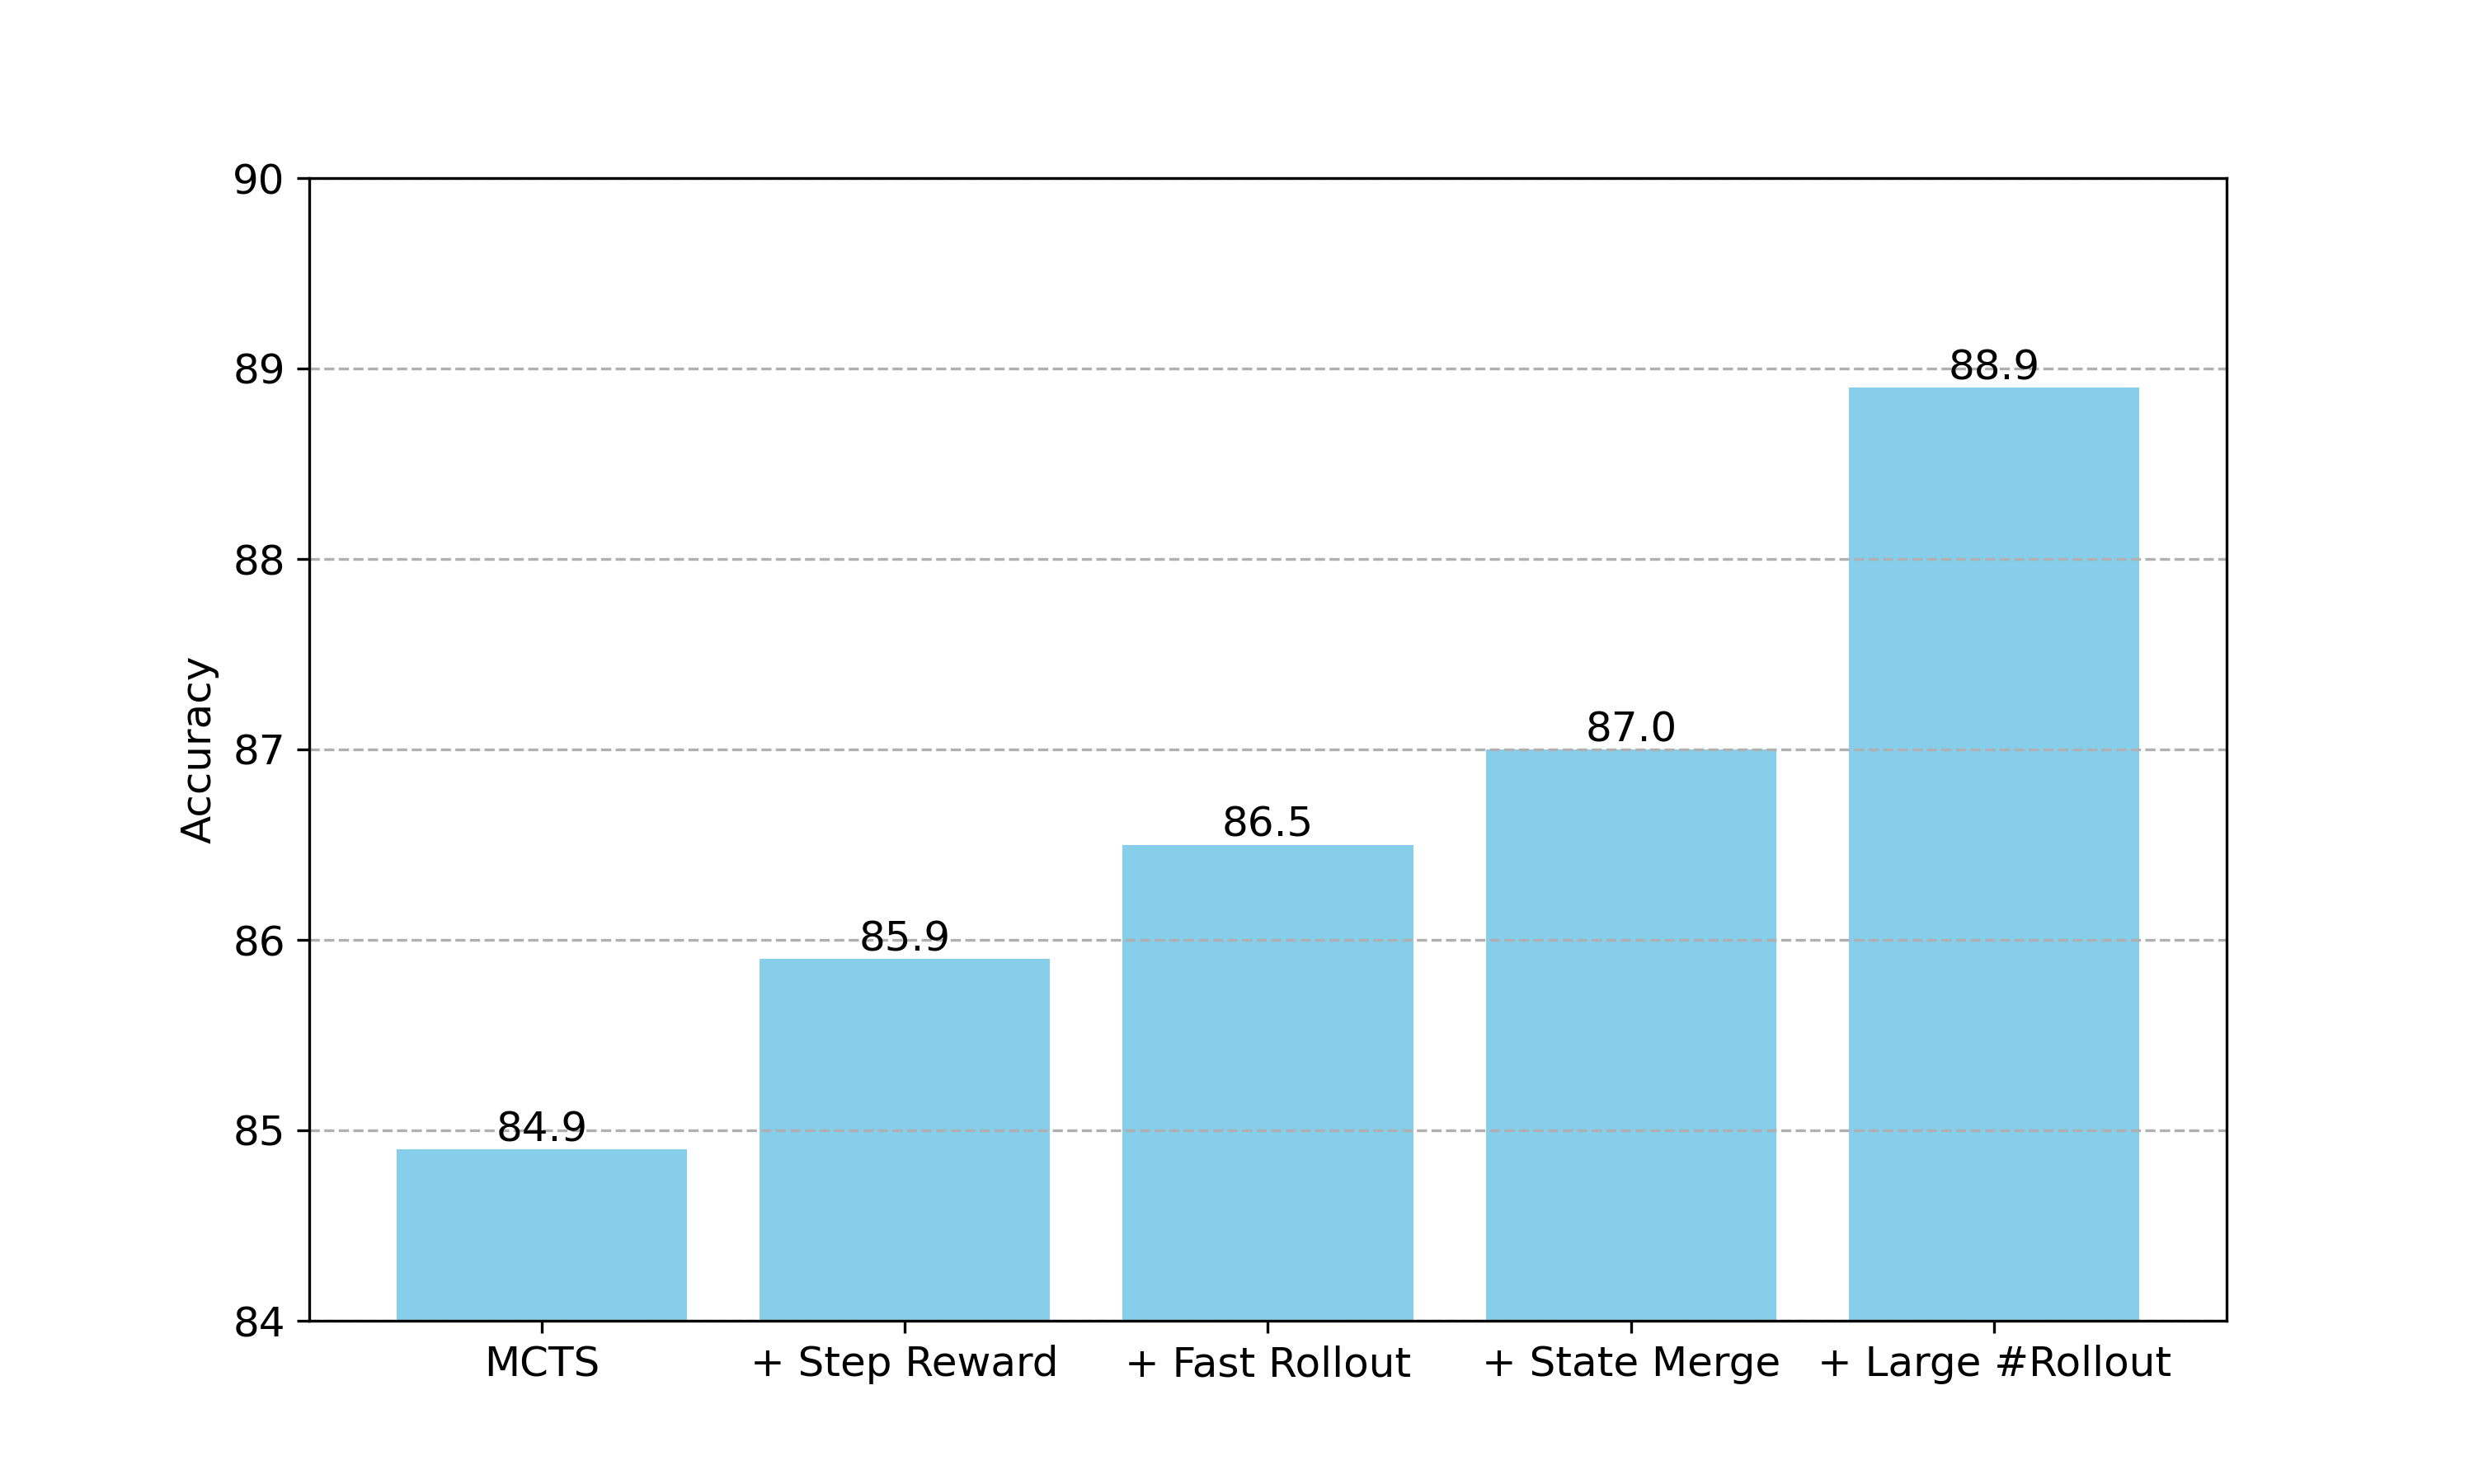
\includegraphics[width=0.75\textwidth]{figures/mcts_ablation.png}
    \caption{Ablation study on the GSM8K test set of various enhancements to the proposed efficient MCTS, including \prm{}, fastrollout with \orm{}, state merging, and increasing the number of rollouts.}
    \label{fig:search_ablation}
\end{figure}


% \begin{figure}[ht]
%     \centering
%     % Minipage for the Table
%     \begin{minipage}{0.25\textwidth}
%         \centering
%         \begin{tabular}{|l|c|}
%             \hline
%             Column 1 & Column 2 \\
%             \hline
%             Item 1 & Item 2 \\
%             Item 3 & Item 4 \\
%             \hline
%         \end{tabular}
%         \caption{Example Table}
%         \label{table:example_table}
%     \end{minipage}
%     \hfill
%     % Minipage for the Figure
%     \begin{minipage}{0.7\textwidth}
%         \centering
%         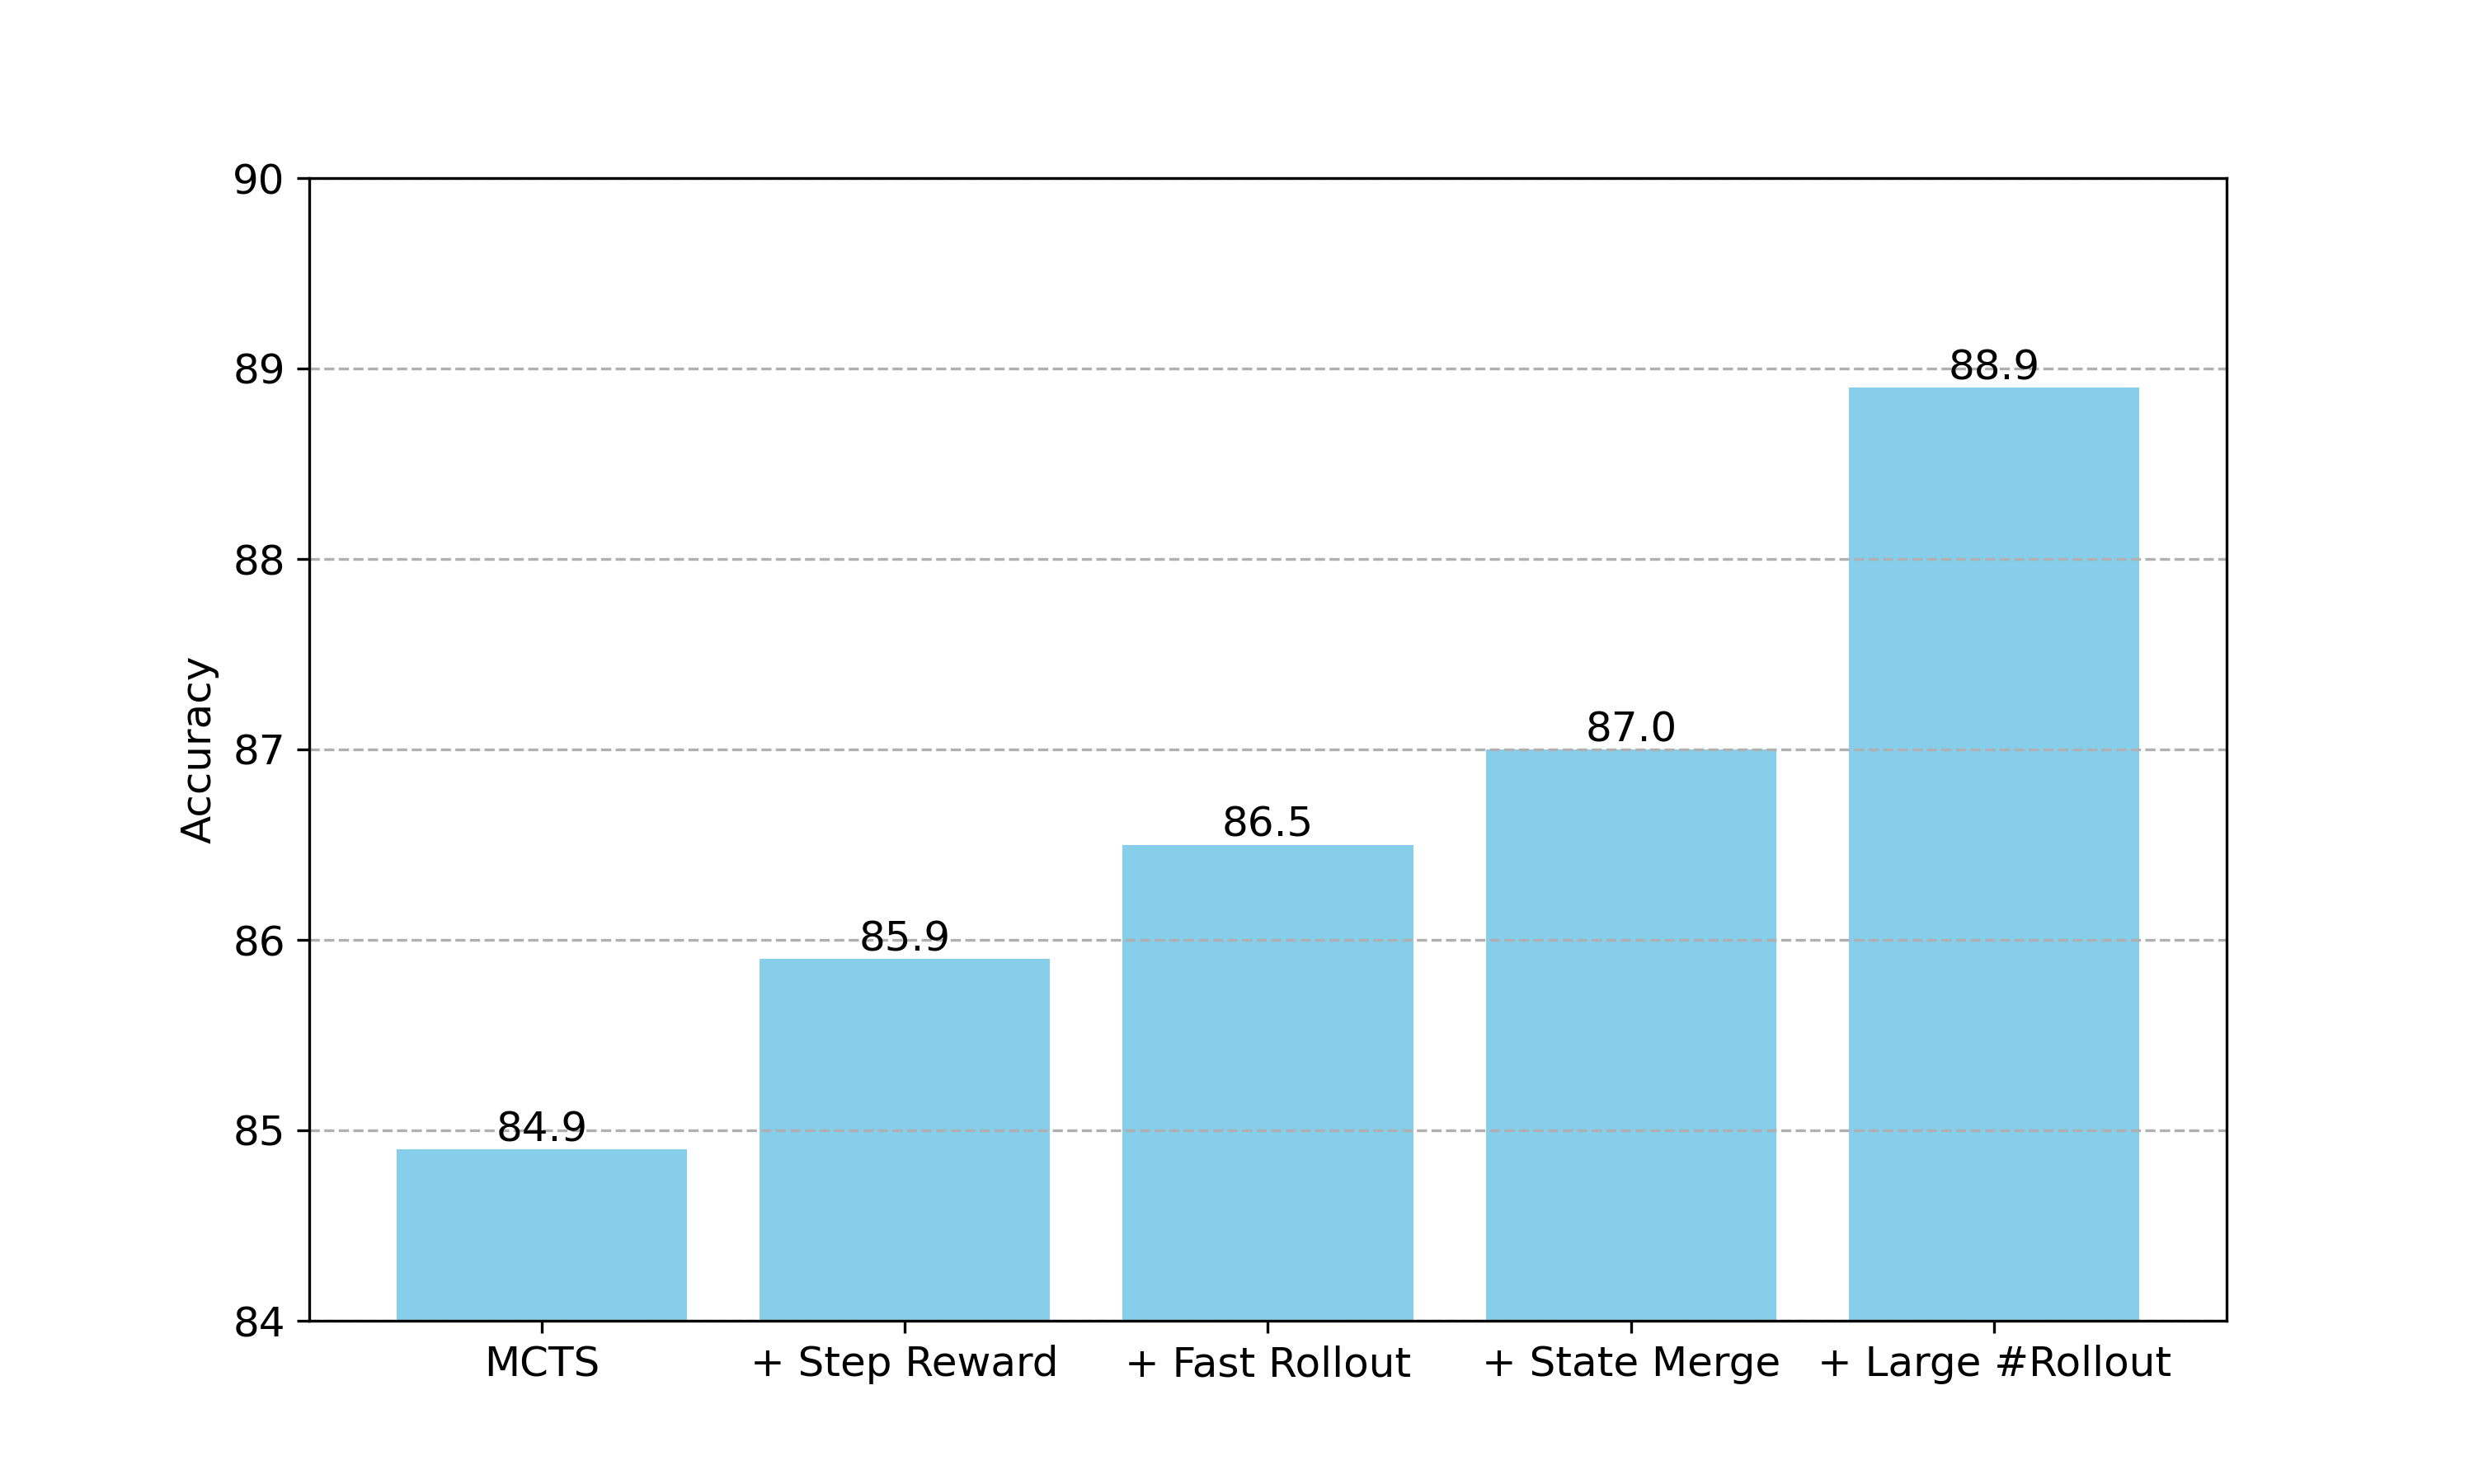
\includegraphics[width=0.9\textwidth]{figures/mcts_ablation.png}
%     \caption{Ablation study on the GSM8K test set of various enhancements to the proposed efficient MCTS, including \prm{}, fastrollout with \orm{}, state merging, and increasing the number of rollouts.}
%     \label{fig:search_ablation}
%     \end{minipage}
% \end{figure}

\begin{table}[h]
\small
\centering
\begin{minipage}{.5\linewidth}
\centering

\begin{tabular}{ccccc|c}
\toprule
\texttt{AB} & \prm{} & \texttt{FR}-\orm{} & \texttt{SM} & \texttt{LG-\#Rollout} & Acc \cr
\midrule
$\times$ & $\times$ & $\times$ & $\times$ & $\times$ & 79.5 \\
$\checkmark$ & $\times$ & $\times$ & $\times$ & $\times$ & 84.9 \\
$\checkmark$ & $\checkmark$ & $\times$ & $\times$ & $\times$ & 85.9 \\
$\checkmark$ & $\checkmark$ & $\checkmark$ & $\times$ & $\times$ & 86.5 \\
$\checkmark$ & $\checkmark$ & $\checkmark$ & $\checkmark$ & $\times$ & 87.0 \\
$\checkmark$ & $\checkmark$ & $\checkmark$ & $\checkmark$ & $\checkmark$ & 88.9 \\
\bottomrule
\end{tabular}
\vspace{2mm}
\caption*{(a) Ablation study on GSM8K}
% \caption{First Table: Ablation study on GSM8K test set.}
\end{minipage}%
\begin{minipage}{.5\linewidth}
\centering

\begin{tabular}{cc|cc}
\toprule
\texttt{TA}-\orm{} & \texttt{Option}  & \texttt{Acc} & \texttt{\#Rollout} \cr
\midrule
$\times$ & $\times$ & 38.8 & 201 \\
$\checkmark$ & $\times$ & 44.1 & 198 \\
$\checkmark$ & $\checkmark$ & 45.4 & 148 \\
\bottomrule
\end{tabular}
\vspace{2mm}
\caption*{(b) Ablation study on MATH}
\end{minipage}
\caption{\textbf{(a)}: Ablation studies on the GSM8K test set of various components of \emcts{}, including adaptive branching, \prm{}, fast-rollout with \orm{}, state merge, and large number of rollouts. \textbf{(b)}: Ablation studies of the impacts of tool-augmented \orm{} and option-level formulation  on MATH.}
\label{table:ablation}
\end{table}


We assess the effectiveness of each component in \model{} and report the results on GSM8K in Table~\ref{table:ablation}(a). Vanilla MCTS, configured with only the value function and a fixed number of children per node, achieves an accuracy of 79.5\%. This serves as a reference point for evaluating the incremental benefits introduced by each additional component. The use of adaptive branching increae the accuracy to 84.9\%. The addition of \prm{} improves the accuracy modestly to 85.9\%, showing the effectivenss of process supervision for searching. A more significant improvement is observed with the introduction of \orm{} with fast rollout, which boosts the accuracy to 86.5\%.  Integrating state merging results in a further increase in accuracy, reaching 87.0\%. Finally the combined of increasing the number of rollouts with the other components yields the best performance on this task. 

Table~\ref{table:ablation}(b) presents the ablation study of option formulation and the tool-augmented critic on the MATH dataset. Our proposed \emcts{} achieves an accuracy of 45.4 with 148 rollouts. When options are excluded, reverting to essentially sentence-level MCTS, the performance decreases to 44.1 with a noticeable increase in the number of rollouts to 198. This demonstrates that option formulation introduces enhanced flexibility to MCTS, enabling better performance with fewer search efforts. Furthermore, the most significant decrease in performance is observed when only intrinsic knowledge is utilized for \orm{}, which drops to an accuracy of 38.8. This suggests that the absence of an external tool critically impedes the \orm{}'s capability to effectively assess challenging math problems.


% \begin{wraptable}{r}{5.5cm}
% \label{tab:option_critic}
% % \vspace{-5mm}

% % \label{tab:my_label}
% \begin{tabular}{lcc}

% \toprule
% Method & \texttt{Acc} & \texttt{\#Rollout} \\
% \midrule
% \emcts{} & 45.4 & 148 \\
% \ w/o option & 44.1 & 198 \\
% \ \orm{} w/o tool  & 38.8 & 201 \\
% \bottomrule

% \end{tabular}
% \caption{Comparison results of options formulation on MATH.}
% \end{wraptable}
\begin{figure}[!tbp]
    \centering
    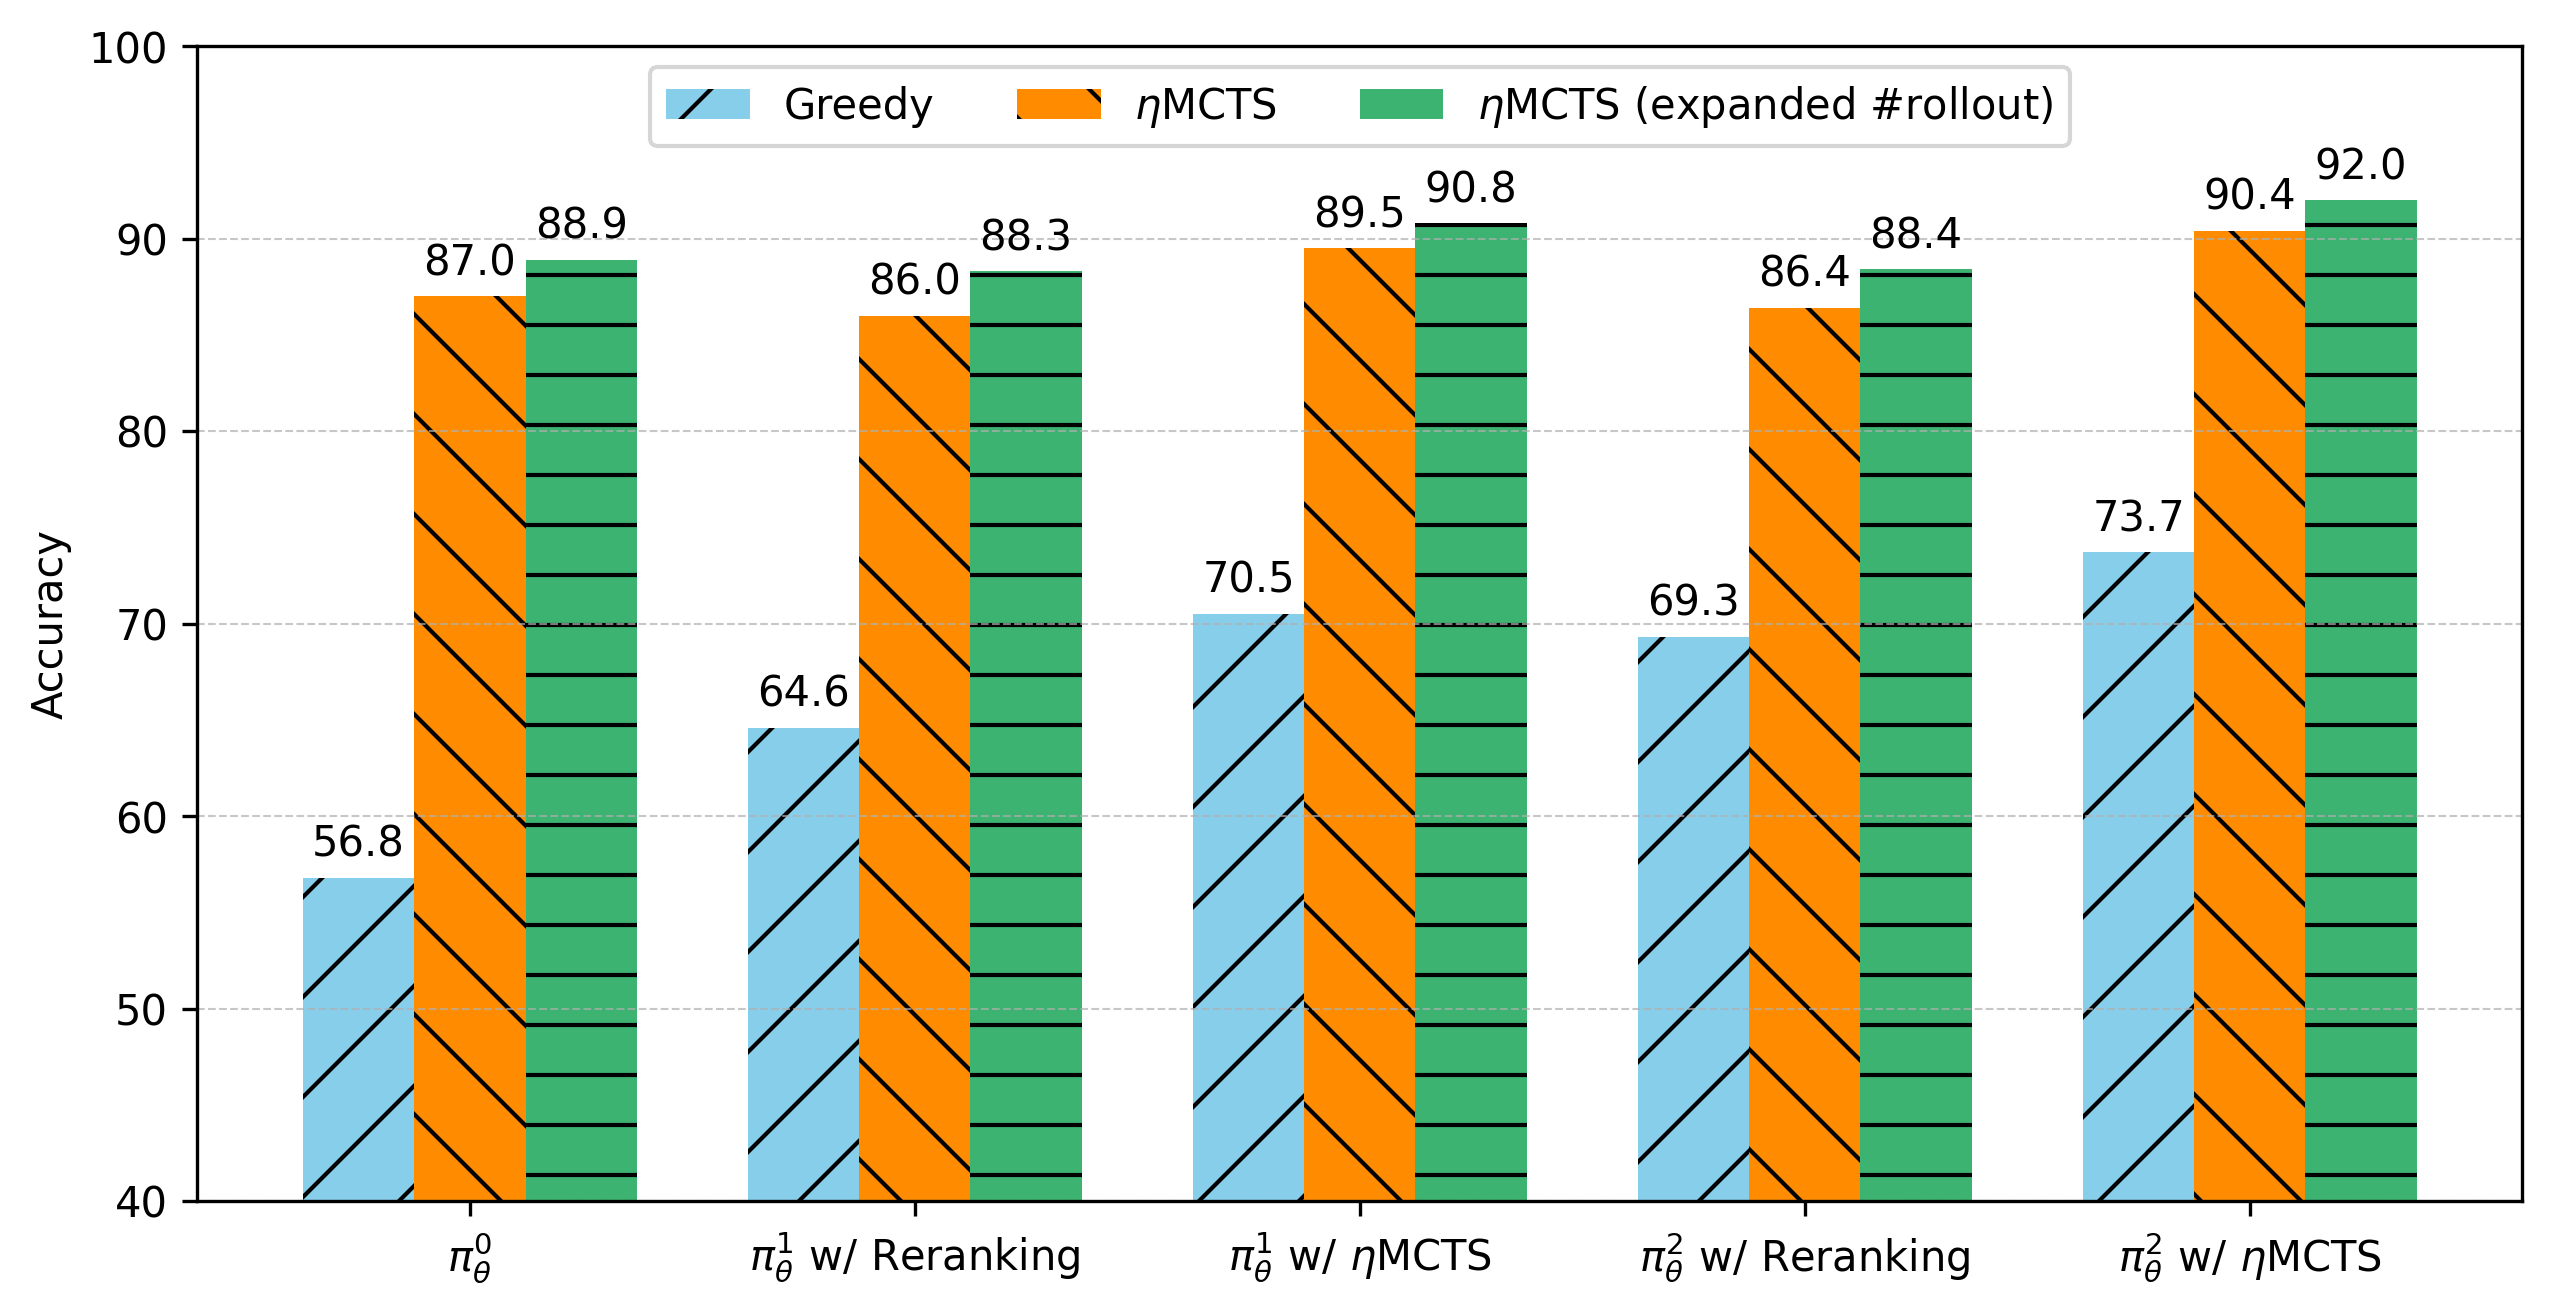
\includegraphics[width=0.9\textwidth]{figures/model_self_improving_n_rounds_results_v2.png}
    \caption{Empirical analysis on GSM8K of different self-improving data collection methods and number of iterations. Models are evaluated with greedy decoding, \emcts{} with small \#rollout and large \#rollout. }
    \label{fig:self_improving_ablations}
\end{figure}
Figure~\ref{fig:self_improving_ablations} depicts a comparative results on GSM8K of two rounds of self-improving trained on trajectories collected using reranking and \emcts{}. We report the performance of greedy decoding, \emcts{} with a relatively small number of rollouts (50-60), and \emcts{} with a larger number of rollouts (200-300) for each model. We observe that 1) Models trained on the trajectories from reranking or \emcts{} outperform the initial policy by a significant margin. In addition, the performance can be iteratively improved with training suggesting that self-improving has the potential to achieve continual performance gain. 2) While both reranking and \emcts{} can generate high-quality trajectories for self-improving , \emcts{} is performant with high efficiency and better accuracy. Models trained on trajectories generated by it not only exceed the performance of those trained on reranked trajectories but also, when decoded with \emcts{}, demonstrate on par performance with GPT-4, revealing that \model{} is an effective self-improving framework.

% 2) ablation study:
% search times, each components


\begin{table}[h]
\small
\centering
\begin{minipage}{.45\linewidth}
\centering

    \begin{tabular}{cl|c|c}
    \toprule
        \multicolumn{2}{c|}{\texttt{Method}}         & \texttt{Threshold}  & \texttt{Acc}\\
        % \hline
        \midrule
           &   Edit distance	               & $20$ & $86.8$ \\
           &   Edit distance	             & $50$ & $87.0$\\
           &  Cosine Similarity	            & $0.7$ & $86.3$\\
           & Model-based	& N/A	& $86.7$ \\
        \bottomrule
    \end{tabular}
\vspace{2mm}
\caption*{(a) Ablation on the choice of state merge functions.}
% \caption{First Table: Ablation study on GSM8K test set.}
\end{minipage}%
\begin{minipage}{.55\linewidth}
\centering

    \begin{tabular}{cl|c}
    \toprule
        \multicolumn{2}{c|}{\texttt{\#Trajetory}}         & \texttt{Acc}\\
        \midrule
           &   $1$	                & $85.9$ \\
           &   $4$	           & $86.5$\\
           &  $8$	       & $86.7$\\
        \bottomrule
    \end{tabular}
\vspace{2mm}
\caption*{(b) Ablation on the number of trajectories.}
\end{minipage}
\caption{\textbf{(a)}: Ablation studies on the choice of heuristic/model-based functions in state merge on GSM8K with base Llama2-70b. The model used in the model-based state merge is Llama-2-70b-chat. \textbf{(b)}: Ablation studies of the number of rollout trajectories in fast-rollout estimation on GSM8K with base Llama2-70b.}
\label{table:ablation_sm}
\end{table}

We further analyze the impact of different hyperparameters and design choices for each component. Table~\ref{table:ablation_sm}(a) shows that varying heuristic functions (with hyperparameters) for state merge has limited impact on performance. Table~\ref{table:ablation_sm}(b) shows that, as the number of fast-rollouts increases, there is a corresponding improvement in performance. This is due to the reduction in the variance of the estimates. We used $n=4$ in our experiments for better trade-off between performance and efficiency. Additional ablations on the choice of fast-rollout models, are provided in Appendix \ref{app:add_ablations}.


% Analysis: 
% x: bin of acc.  y: avg step/outcome reward
% value acc. for fast-rollout vs no fast-rollout
% Tool use vs. no tool use on MATH set (v$_2$ small vs. v$_4$ small)

% \subsection{Self-improving Results}



